%standard 4.3

%start_of_questions

%new_question
%%%%%%%%%%%%%%%%%%%%%
	% Problem 9
	% Difficulty: 3
%%%%%%%%%%%%%%%%%%%%%
	\item  
		%https://edabit.com/challenge/xR248CxGSsSrNK5Za
		You are the newest rug fashion designer on the scene, but you're running out of ideas. 
		Write a program that will help you design rugs.  The program should ask for a width, 
		a length, and pattern, and then create a rug consisting of that pattern and dimensions.

		For example, \\ \ \hfill
		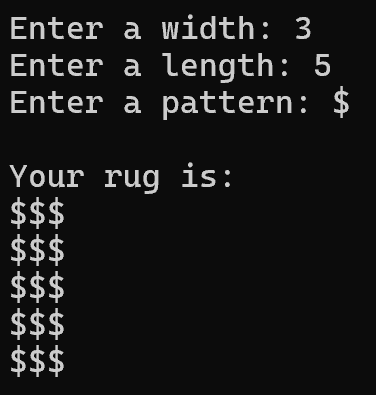
\includegraphics[width = 1.5in]{./imgs/rug1.PNG} \hfill  
		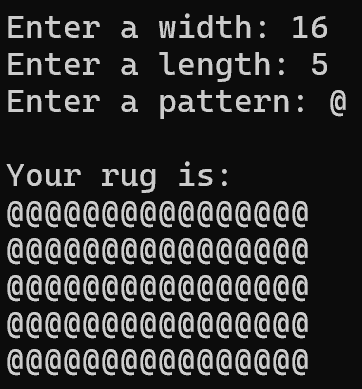
\includegraphics[width = 1.5in]{./imgs/rug2.PNG} \hfill \


%new_question
%%%%%%%%%%%%%%%%%%%%%
	% Problem 12
	% Difficulty: 3
%%%%%%%%%%%%%%%%%%%%%
	\item   
		Ask the user for two integer, and then build a multiplication table based on those numbers.

		For example, \\ \ \hfill
		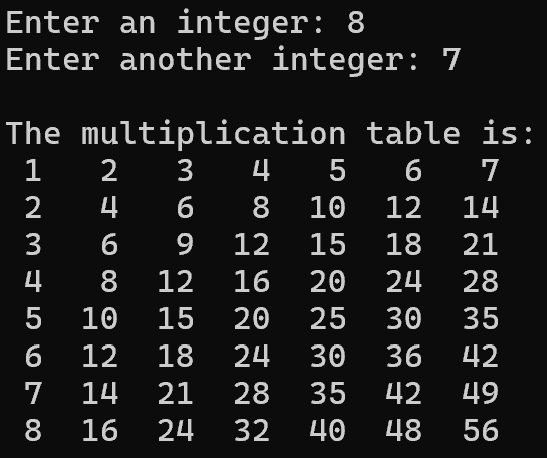
\includegraphics[height = 1.5in]{./imgs/mult_table1.PNG} \hfill  
		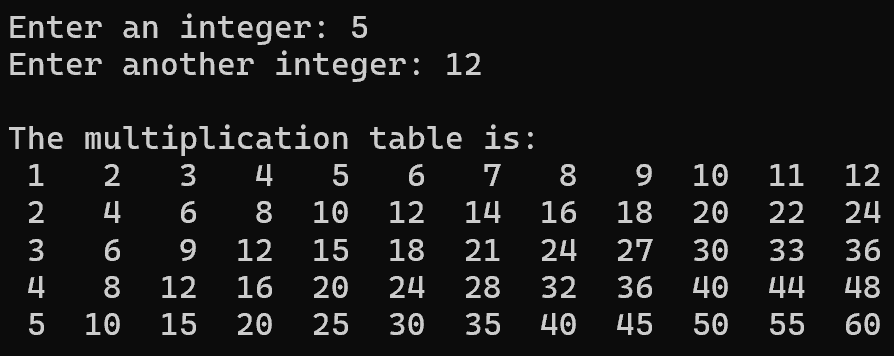
\includegraphics[height = 1.2in]{./imgs/mult_table2.PNG} \hfill  \


%new_question
%%%%%%%%%%%%%%%%%%%%%
	% Problem 13
	% Difficulty: 3
%%%%%%%%%%%%%%%%%%%%%
	\item  
		Ask the user for an integer height, and then build a triangle of asterisks (*) 
		with that height.

		For example, \\ \ \hfill
		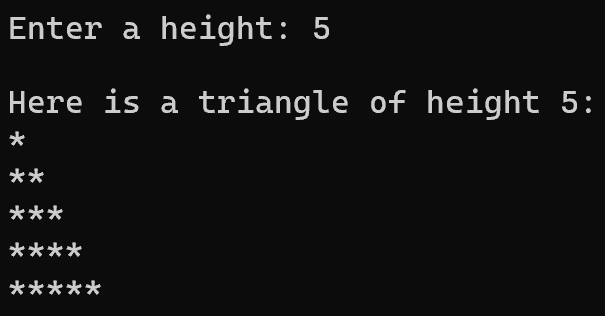
\includegraphics[height = 1.2in]{./imgs/triangle1.PNG} \hfill  
		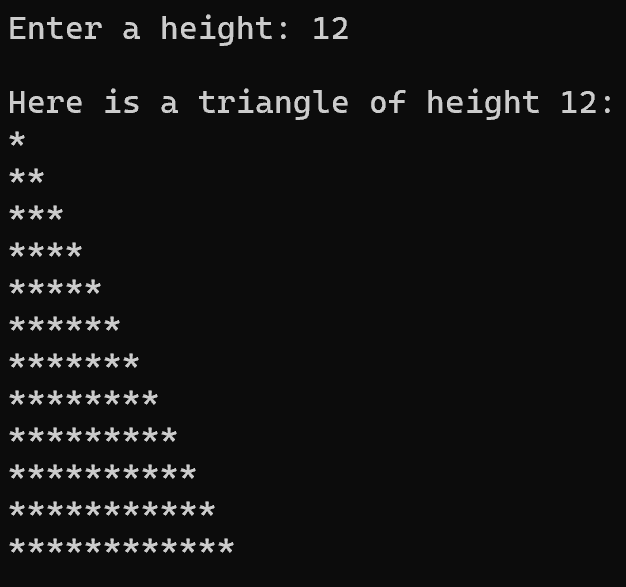
\includegraphics[height = 1.4in]{./imgs/triangle2.PNG} \hfill  \

%end_of_questions

